%%%%%%%%%%%%%%%%%%%%%%%%%%%%%%%%%%%%%%%%%
% Beamer Presentation
% LaTeX Template
% Version 1.0 (10/11/12)
%
% This template has been downloaded from:
% http://www.LaTeXTemplates.com
%
% License:
% CC BY-NC-SA 3.0 (http://creativecommons.org/licenses/by-nc-sa/3.0/)
%
%%%%%%%%%%%%%%%%%%%%%%%%%%%%%%%%%%%%%%%%%

%----------------------------------------------------------------------------------------
%	PACKAGES AND THEMES
%----------------------------------------------------------------------------------------

\documentclass{beamer}

\mode<presentation> {

% The Beamer class comes with a number of default slide themes
% which change the colors and layouts of slides. Below this is a list
% of all the themes, uncomment each in turn to see what they look like.

%\usetheme{default}
%\usetheme{AnnArbor}
%\usetheme{Antibes}
%\usetheme{Bergen}
%\usetheme{Berkeley}
%\usetheme{Berlin}
%\usetheme{Boadilla}
%\usetheme{CambridgeUS}
%\usetheme{Copenhagen}
%\usetheme{Darmstadt}
%\usetheme{Dresden}
\usetheme{Frankfurt}
%\usetheme{Goettingen}
%\usetheme{Hannover}
%\usetheme{Ilmenau}
%\usetheme{JuanLesPins}
%\usetheme{Luebeck}
%\usetheme{Madrid}
%\usetheme{Malmoe}
%\usetheme{Marburg}
%\usetheme{Montpellier}
%\usetheme{PaloAlto}
%\usetheme{Pittsburgh}
%\usetheme{Rochester}
%\usetheme{Singapore}
%\usetheme{Szeged}
%\usetheme{Warsaw}

% As well as themes, the Beamer class has a number of color themes
% for any slide theme. Uncomment each of these in turn to see how it
% changes the colors of your current slide theme.

%\usecolortheme{albatross}
%\usecolortheme{beaver}
%\usecolortheme{beetle}
%\usecolortheme{crane}
%\usecolortheme{dolphin}
%\usecolortheme{dove}
%\usecolortheme{fly}
%\usecolortheme{lily}
%\usecolortheme{orchid}
%\usecolortheme{rose}
\usecolortheme{seagull}
%\usecolortheme{seahorse}
%\usecolortheme{whale}
%\usecolortheme{wolverine}

%\setbeamertemplate{footline} % To remove the footer line in all slides uncomment this line
%\setbeamertemplate{footline}[page number] % To replace the footer line in all slides with a simple slide count uncomment this line

%\setbeamertemplate{navigation symbols}{} % To remove the navigation symbols from the bottom of all slides uncomment this line
}

\usepackage{graphicx} % Allows including images
\usepackage{booktabs} % Allows the use of \toprule, \midrule and \bottomrule in tables

%----------------------------------------------------------------------------------------
%	TITLE PAGE
%----------------------------------------------------------------------------------------

\title[Spin Systems]{Informational Analysis of Monte Carlo Simulations of Spin Systems} % The short title appears at the bottom of every slide, the full title is only on the title page

\author{Galina Malovichko} % Your name
\institute[UC Davis] % Your institution as it will appear on the bottom of every slide, may be shorthand to save space
{
University of California, Davis \\ % Your institution for the title page
\medskip
\textit{gmalovichko@ucdavis.edu} % Your email address
}
\date{\today} % Date, can be changed to a custom date

\begin{document}

\begin{frame}
\titlepage % Print the title page as the first slide
\end{frame}

% \begin{frame}
% \frametitle{Overview} % Table of contents slide, comment this block out to remove it
% \tableofcontents % Throughout your presentation, if you choose to use \section{} and \subsection{} commands, these will automatically be printed on this slide as an overview of your presentation
% \end{frame}

%----------------------------------------------------------------------------------------
%	PRESENTATION SLIDES
%----------------------------------------------------------------------------------------

%------------------------------------------------
\section{Ising Model} % Sections can be created in order to organize your presentation into discrete blocks, all sections and subsections are automatically printed in the table of contents as an overview of the talk
%------------------------------------------------

\begin{frame}
\frametitle{Ising Model}

$$ H = -J \sum_{\langle i, j \rangle}{S_i S_j} $$\\~\\

\begin{figure}
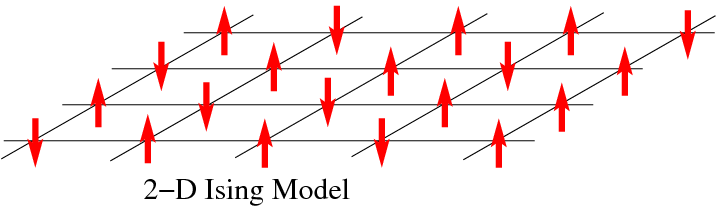
\includegraphics[width=0.8\linewidth]{ising.png}
\end{figure}

\end{frame}

%------------------------------------------------

\begin{frame}
\frametitle{Update algorithm}

\begin{itemize}
\item Flip random spin
\item Find energy change $\Delta E$
\item Keep the spin flipped with probability $p = \frac{1}{1 + \exp{\frac{\Delta E}{T}}}$

\end{itemize}
\end{frame}

%------------------------------------------------
\section{Thermodynamic properties}
%------------------------------------------------

\begin{frame}
\frametitle{Energy vs Temperature}

\begin{figure}
\includegraphics[width=0.8\linewidth]{2D__E_vs_T.png}
\end{figure}

\end{frame}

%------------------------------------------------

\begin{frame}
\frametitle{Magnetization vs Temperature}

\begin{figure}
\includegraphics[width=0.8\linewidth]{2D__M_vs_T.png}
\end{figure}

\end{frame}

%------------------------------------------------

\begin{frame}
\frametitle{Entropy vs Temperature}

$$ S(\beta) = E \beta - \int_0^{\beta} E d\beta $$ 

\begin{figure}
\includegraphics[width=0.8\linewidth]{2D__S_vs_T.png}
\end{figure}

\end{frame}

%------------------------------------------------

\begin{frame}
\frametitle{Entropy and Entropy rate}

\begin{figure}
\includegraphics[width=0.8\linewidth]{2D__hmu_and_S_vs_T.png}
\end{figure}

\end{frame}

%------------------------------------------------
\section{Other lattices}
%------------------------------------------------

\begin{frame}
\frametitle{Other lattices}

\begin{figure}
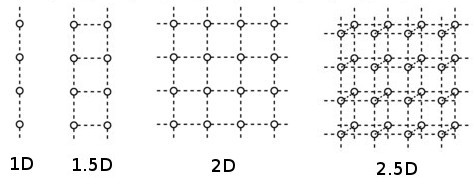
\includegraphics[width=0.8\linewidth]{lattices.jpg}
\end{figure}

\end{frame}

%------------------------------------------------

\begin{frame}
\frametitle{Energies vs Temperature}

\begin{figure}
\includegraphics[width=0.8\linewidth]{all__E_vs_T.png}
\end{figure}

\end{frame}

%------------------------------------------------

\begin{frame}
\frametitle{Magnetizations vs Temperature}

\begin{figure}
\includegraphics[width=0.8\linewidth]{all__M_vs_T.png}
\end{figure}

\end{frame}

%------------------------------------------------

\begin{frame}
\frametitle{Entropies vs Temperature}

\begin{figure}
\includegraphics[width=0.8\linewidth]{all__S_vs_T.png}
\end{figure}

\end{frame}

%------------------------------------------------

\begin{frame}
\frametitle{Entropies and Entropy rates}

\begin{figure}
\includegraphics[width=0.8\linewidth]{all__hmu_and_S_vs_T.png}
\end{figure}

\end{frame}

%------------------------------------------------
\section{Critical temperature}
%------------------------------------------------

\begin{frame}
\frametitle{Critical temperature}

Magnetic susceptibility diverges at critical temperature

\begin{figure}
\includegraphics[width=0.8\linewidth]{2D__X_vs_T.png}
\end{figure}

\end{frame}

%------------------------------------------------

\begin{frame}
\frametitle{Specific Heat}

\begin{figure}
\includegraphics[width=0.8\linewidth]{2D__C_vs_T.png}
\end{figure}

\end{frame}

%------------------------------------------------

\begin{frame}
\frametitle{Binder Cumulant}

$$ B = 1 - \frac{\langle M^4 \rangle}{3 \langle M^2 \rangle ^2} $$

\begin{figure}
\includegraphics[width=0.8\linewidth]{2D__B_vs_T.png}
\end{figure}

\end{frame}

%------------------------------------------------

\begin{frame}
\frametitle{Binder Cumulant}

$$ B = 1 - \frac{\langle M^4 \rangle}{3 \langle M^2 \rangle ^2} $$

\begin{figure}
\includegraphics[width=0.8\linewidth]{2D__B_vs_T_zoom.png}
\end{figure}

\end{frame}

%------------------------------------------------

\begin{frame}
\frametitle{Excess Entropy}

\begin{figure}
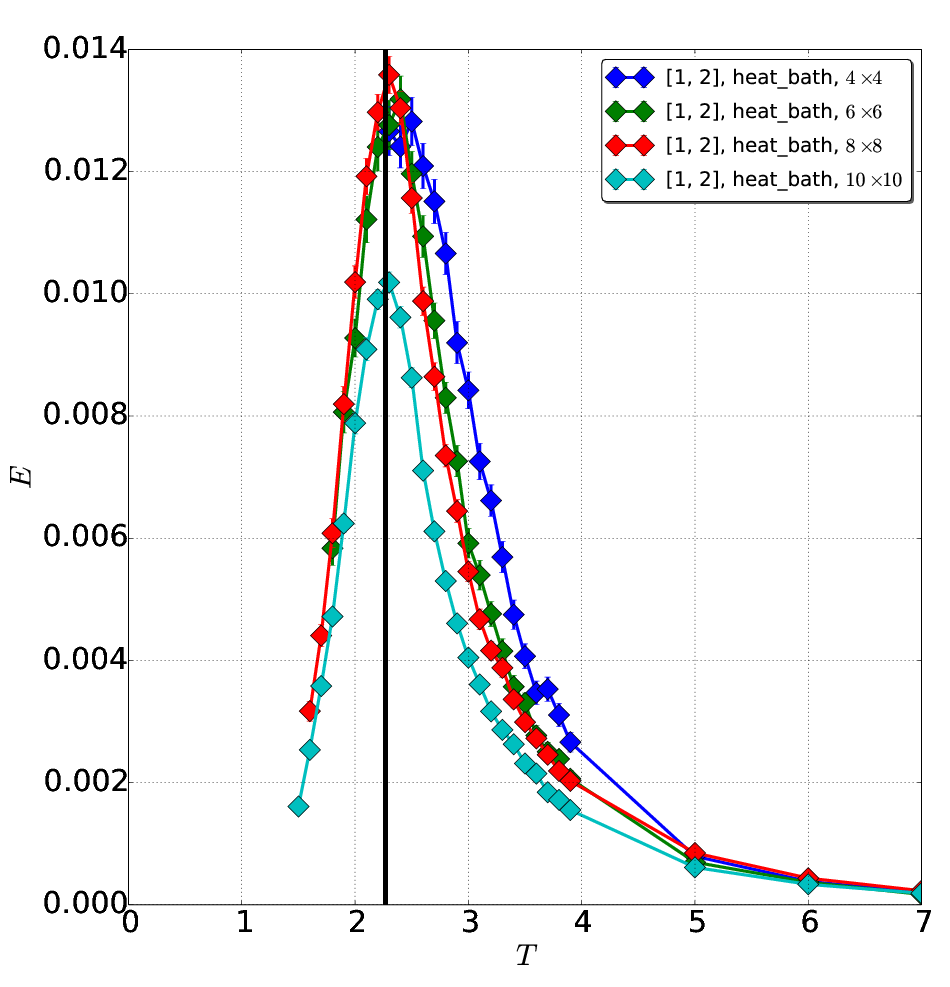
\includegraphics[height=0.6\linewidth]{vlad.png}
\end{figure}

\end{frame}

%------------------------------------------------

%----------------------------------------------------------------------------------------

\end{document}